For the reproducibility purpose, the MATLAB code and datasets used to produce the numerical results in this section are available online at \url{https://github.com/AdMeynard/BoundaryEffectsReduction}.


\subsection{Extension Methods for Comparison}
\label{sse:methods}
To highlight the fact that the linear dynamical model is sufficient to catch most of the dynamical behavior of signals following the AHM, we compare the performance of Algorithm~\ref{alg:boundary} with a simple extension obtained by pointwise symmetrization~\cite{Kharitonenko02wavelet}. We also evaluate the performance of reference forecasting algorithms that could be used for extending such signals. These methods are:
\begin{itemize}
\item The EDMD has been developed by Williams \etal~\cite{Williams15data}. The proposed algorithm is a way to obtain an approximation of the so-called Koopman operator of the observed system, which theoretically allows catching dynamic of nonlinear systems~\cite{Korda18linear}.
\item The GPR~\cite{Rasmussen06gaussian} is a method relying on a probabilistic dynamical model. That one is based on the Gaussian process structure, and therefore offers more flexibility in the type of dynamic that could be modeled than the linear model~\eqref{eq:dyn.model}.
\item The TBATS method~\cite{DeLivera11forecasting} is based on a classical decomposition of times series into a trend, seasonal and ARMA components, with a specific dynamic for the seasonal component. This model demands the estimation of numerous parameters and, by implication, may require a long computation time.
\end{itemize}


\subsection{Evaluation Metrics}

The first evaluation metric is quantifying the forecasting quality (\ie~not depending on $\ell$) in the time domain. We evaluate the Experimental Mean Square Error $\mathrm{MSE_{xp}}(\tilde\bx)$ of the forward forecast extended signals, namely,
\begin{align}
\label{eq:mse}
\mathrm{MSE_{\xp}}(\tilde\bx) &= \dfrac1{L}\|\tilde\bx -\bx^\mathrm{ext}\|^2 \\[-1mm]
\nonumber
&=\! \dfrac1{L}\sum_{\ell=1}^L \bmu_{\xp}[N\!-\!1\!+\!\ell]^2 \!+\! \bgamma_{\xp}[N\!-\!1\!+\!\ell,N\!-\!1\!+\!\ell] .
\end{align}
where $\bx^\mathrm{ext}$ is the {\em ground-truth extended} signal; that is, $\bx^\mathrm{ext} := \begin{pmatrix}\bx[-L] & \cdots & \bx[N-1+L] \end{pmatrix}$. Then, as long as the bias $\bmu[N-1+\ell]$ and the variance $\bgamma[N-1+\ell,N-1+\ell]$ of the forecasting estimator remain small for all $\ell$, the MSE takes small values either.



The second evaluation metric is evaluating the quality of the boundary effect reduction directly on the TF representation. We compare the obtained TF representation to the optimal TF representation $\ccF_N^\mathrm{opt}(\bx)$, defined as the restriction of the representation of the ground-truth extended signal $\bx^\mathrm{ext}$; that is, we have
\begin{equation}
\ccF^\mathrm{opt}(\bx_N) = \cR\left( \ccF(\bx^\mathrm{ext}) \right) \, ,
\label{eq:opt.TFR}
\end{equation} 
where $\mathcal{R}$ is defined in \eqref{eq:bound.free.TFR}.
To compare different techniques, we use a criterion proposed in~\cite{Daubechies16conceft} that quantifies the optimal transport (OT) distance between a given TF representation and the optimal one. In general, the OT distance is a quantity that measures how different two probability density functions are. Denote a TF representation as $\ccQ$. For $t$ fixed, we consider the probability density function defined by $p_\ccQ^t(\xi) = \left. |\ccQ(\xi,t)|^2 \middle/ \int_\RR |\ccQ(\nu,t)|^2\dd\nu \right.$; that is, normalizing the spectral information at time $t$. At each time $t$, the OT distance $d_{t}$ between two TF representations $\ccQ$ and $\ccF^\mathrm{opt}$ at time $t$ is defined by
\begin{equation*}
d_{t}(\ccQ,\ccF^\mathrm{opt}) = \int_\RR\left|\tilde P_{\ccQ}^t(\xi)-  P_{\ccF^\mathrm{opt}}^t(\xi)\right|\dd\xi\ ,
\end{equation*}
where $P_{\ccQ}^t(\xi)=\int_{-\infty}^\xi p_{\ccQ}^t(\nu)\dd\nu$ and $\tilde P_{\ccF^\mathrm{opt}}^t(\xi)=\int_{-\infty}^\xi\tilde p_{\ccF^\mathrm{opt}}^t(\nu)\dd\nu$. In other words, the OT distance between $\ccQ$ and $\ccF^\mathrm{opt}$ at time $t$ is given by the $L^1$ norm of the associated cumulative density function.  %
Note that $d_{t}(\ccQ,\ccF^\mathrm{opt})$ quantifies the proximity between the estimated and actual TF representations at time $t$. With the OT distance, we define the {\em performance index} $D(\ccQ,\ccF)$ for the reduction of boundary effects of a given TF representation $\ccQ$ over another TF representation $\ccF$ by
%\begin{equation}
%D(\ccQ) = \dfrac1{|I|}\bigintssss_I\ \frac{d_{t}\left(\ccQ,\ccF^\mathrm{opt}\right)}{d_{t}\left(\ccF,\ccF^\mathrm{opt}\right)}\ \dd t\ .
%\label{eq:index.perf}
%\end{equation}
\begin{equation}
D(\ccQ,\ccF) = \dfrac{\displaystyle\int_I d_{t}\left(\ccQ,\ccF^\mathrm{opt}\right)\dd t}{\displaystyle\int_I d_{t}\left(\ccF,\ccF^\mathrm{opt}\right)\dd t}\ .
\label{eq:index.perf}
\end{equation}
In other words, $D(\ccQ,\ccF)$ is the ratio between its averaged OTD to the optimal TF representation $\ccF^\mathrm{opt}$ (see~\eqref{eq:opt.TFR}) and the averaged OTD of the original TF representation $\ccF$ to $\ccF^\mathrm{opt}$.
%
Thus, $D(\ccQ)<1$ means a reduction of the boundary effects. Let us evaluate the quality of the boundary effects reduction on biomedical signals.


\subsection{Simulated Signals}
We first evaluate the quality of the forecasting step and compare it to the theoretical results provided by Theorem~\ref{th:error}. The level of the forecasting error depends on at least two parameters:
\begin{itemize}
\item The noise variance $\sigma^2$.
\item The size of the training dataset $K$. 
\end{itemize}
In subsections~\ref{ssse:res.sine} and~\ref{ssse:res.ahm}, we study the influence of these parameters. A comparison with the theoretical results of section~\ref{se:theoretical} is also available.

\subsubsection{Sum of sine waves}
\label{ssse:res.sine}
We proved that the linear dynamic model is sufficient to catch the dynamical behavior of signals taking the form~\eqref{eq:sum.sine}. In order to validate this theoretical result, we apply the forecasting Algorithm~\ref{alg:extension} to a large number of realizations of the random vector $\bx$ of size $N=10^4$, following model~\eqref{eq:model.noise}, and such that the deterministic component $\bz$ takes the form:
\[
\bz[n]\! =\!\cos\!\left(2\pi p_1 \dfrac{n}{M} \right)\! +\! A\cos\!\left(2\pi p_2 \dfrac{n}{M} \right),\quad \!\!\forall n\!\in\!\{1,\ldots,N\},
\]
with $M=150$, $p_1=10$, $p_2=33$ and $A=1.4$. Besides, the additive noise is chosen to be Gaussian: $\bw\sim\cN(\bzero,\bI)$.


\paragraph{Influence of the Noise Variance $\sigma^2$} Here, the size of the training dataset is set to $K=450$. Then, the forecasting algorithm is run on $500$ realizations on the discrete signal $\bx$ for $200$ different values of $\sigma$, logarithmically equispaced from $10^{-7}$ to $10^{-1}$. For each of these values, we determine the experimental bias, denoted as $\mu_{\xp}[N-1+\ell]$, and experimental variance, denoted as $\gamma_{\xp}[N-1+\ell,N-1+\ell]$. Fig.~\ref{fig:res.noise.sine} shows the experimental forecasting variance as a function of the noise variance for three different values the forecasting sample index: $\ell=1$, $\ell=10$, and $\ell=100$.

\begin{figure}
\centering
%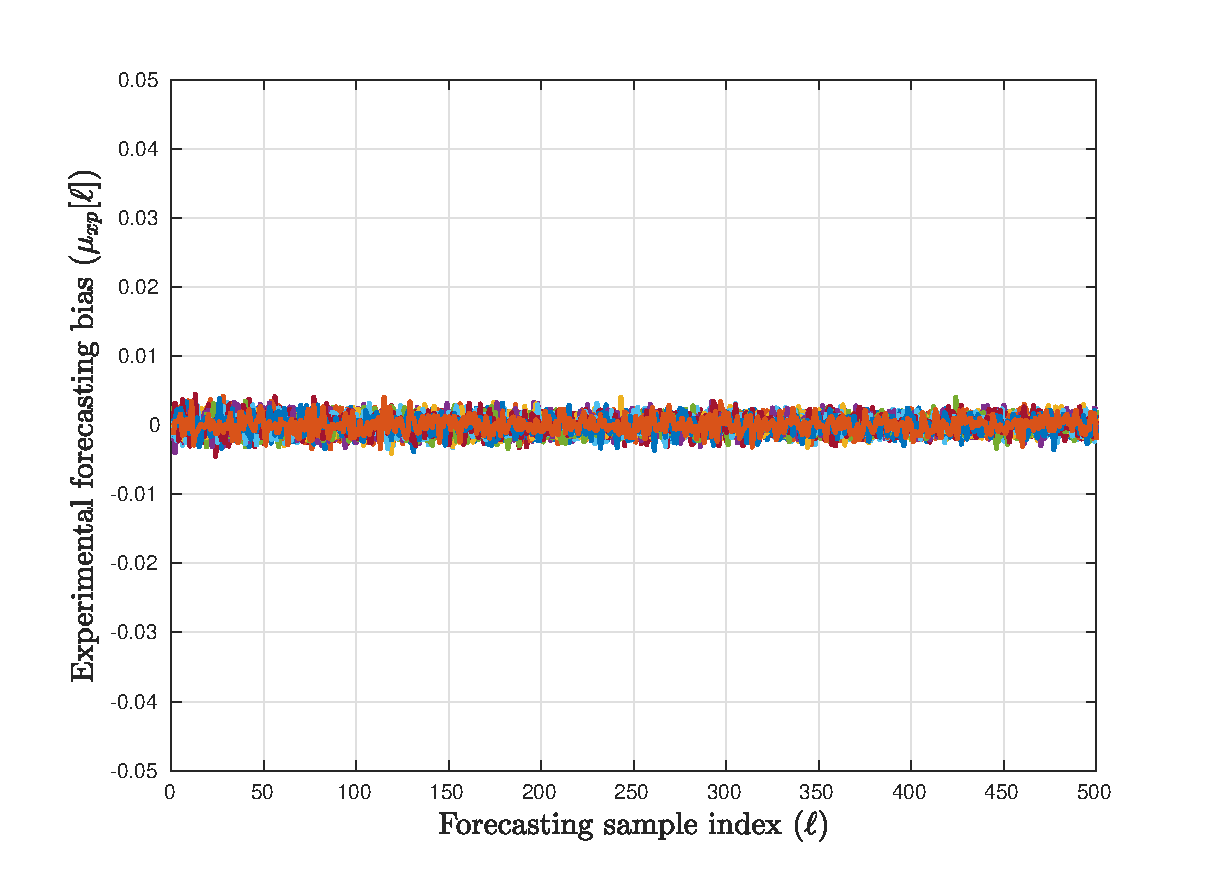
\includegraphics[width=.24\textwidth]{biasNoiseSine.eps}
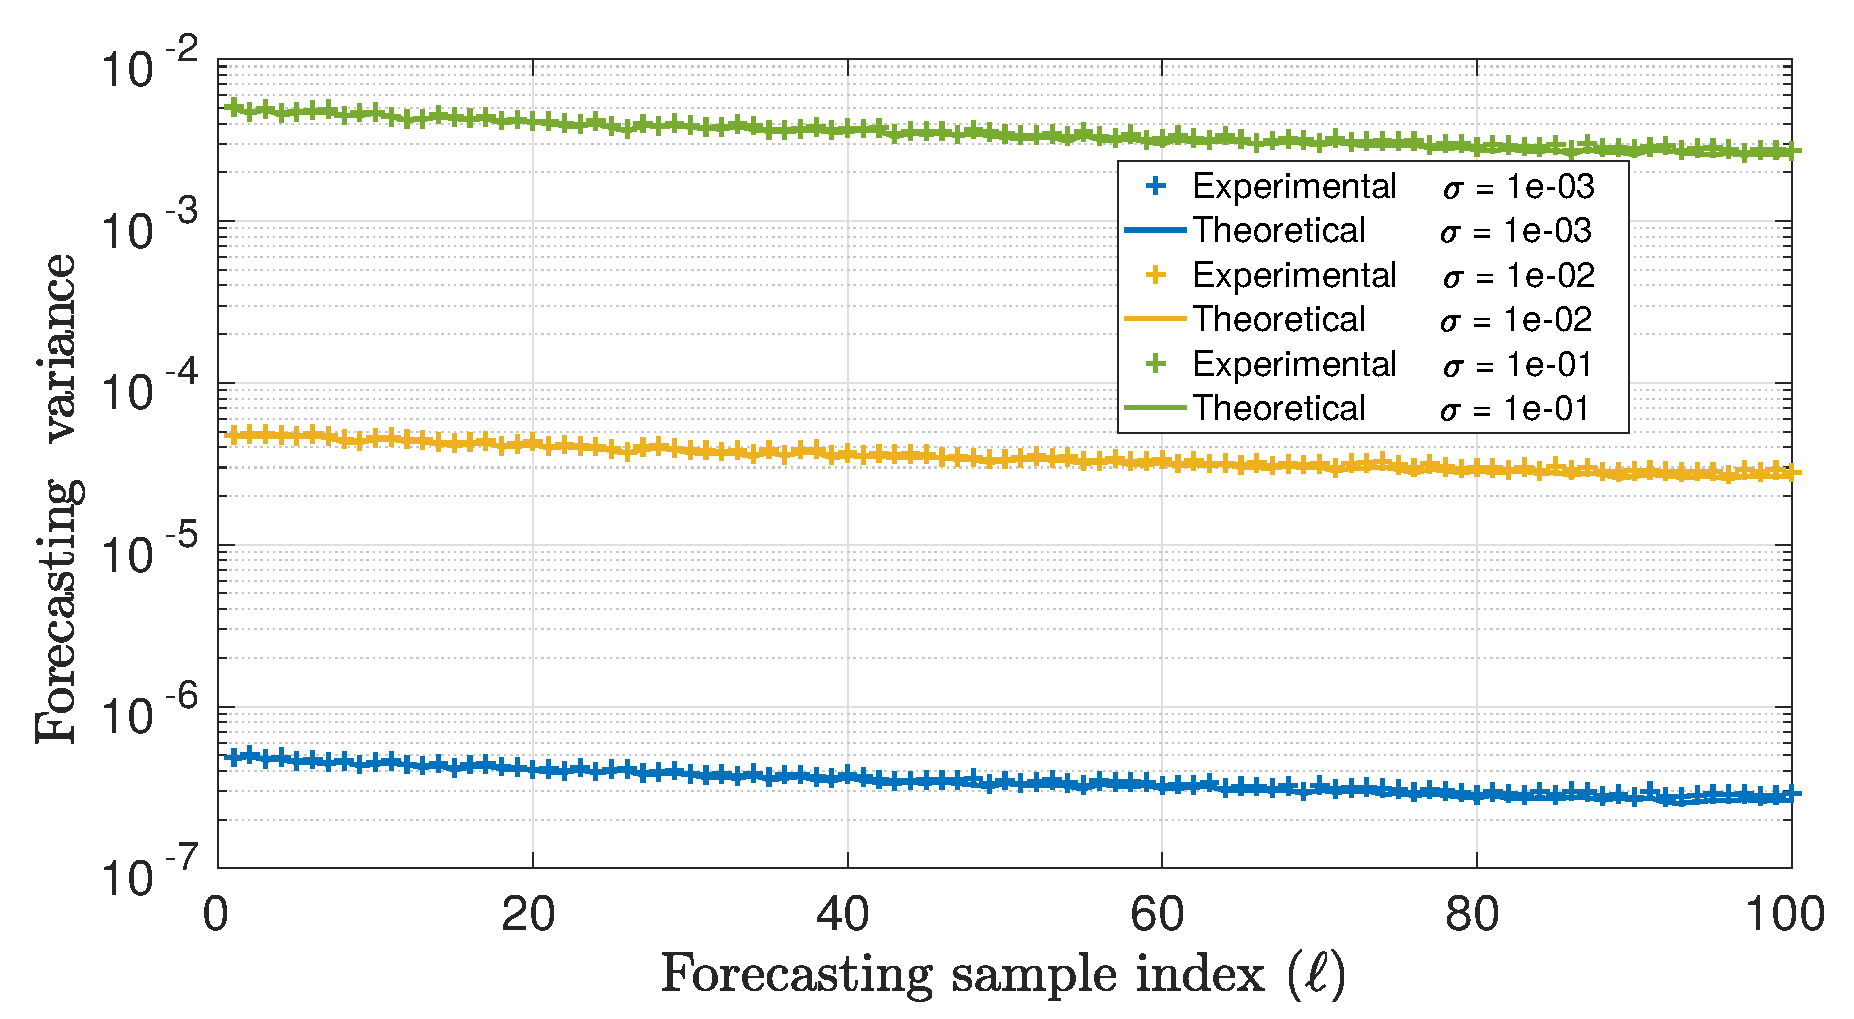
\includegraphics[width=.48\textwidth]{VarianceNoiseSine.eps}
\caption{Evolution of the experimental forecasting variance as a function of the noise variance for three different values the forecasting sample index $\ell$.}
\label{fig:res.noise.sine}
\end{figure}

First, when the noise is weak, the variance of the forecasting estimator is dramatically high. For instance, in this specific example, the estimator $\tilde\bx[N-1+\ell]$ for $\ell=10$ is inaccurate as soon as the noise variance $\sigma^2$ is lower than $4\times 10^{-14}$ (see the red line in Fig.~\ref{fig:res.noise.sine}). This validates the result of Theorem~\ref{th:error}, highlighting the necessary presence of noise to ensure the numerical stability of the estimator. Furthermore, as soon as $\sigma^2$ is higher than this critical threshold, the estimator variance increases linearly with $\sigma^2$, as predicted by the bound~\eqref{eq:cov.error.2} provided in Theorem~\ref{th:error}. Note that the parameter $\ell$ has little influence on the quality of the estimator. This is due to the \textit{stationarity} of the studied signal, allowing long-range forecasts without deterioration of the estimator.

\paragraph{Influence of the Training Dataset Size $K$} Here, the noise variance $\sigma$ is set to $\sigma=10^{-2}$. Then, {\sf SigExt} is run on $500$ realizations of the discrete signal $\bx$ for $200$ different values of training dataset size $K$, logarithmically equispaced from $450$ to $2000$. For each of these values, we determine the experimental bias $\mu_{\xp}[N-1+\ell]$ and variance $\gamma_{\xp}[N-1+\ell,N-1+\ell]$. Fig.~\ref{fig:res.size.sine} shows the experimental forecasting variance as a function of the training dataset size for three different values the forecasting sample index: $\ell=1$, $\ell=10$, and $\ell=100$.

\begin{figure}
%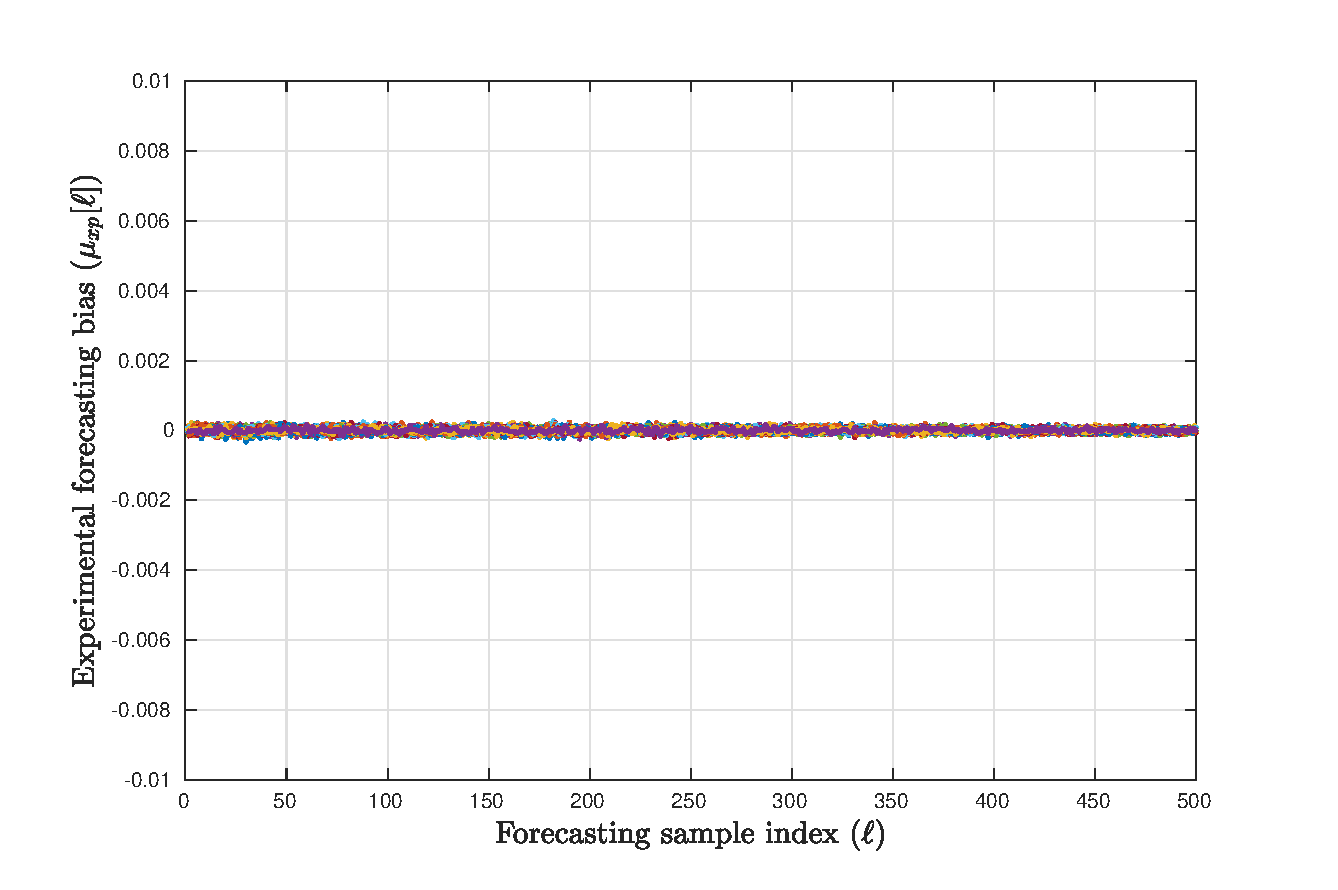
\includegraphics[width=.24\textwidth]{BiasKSine.eps}
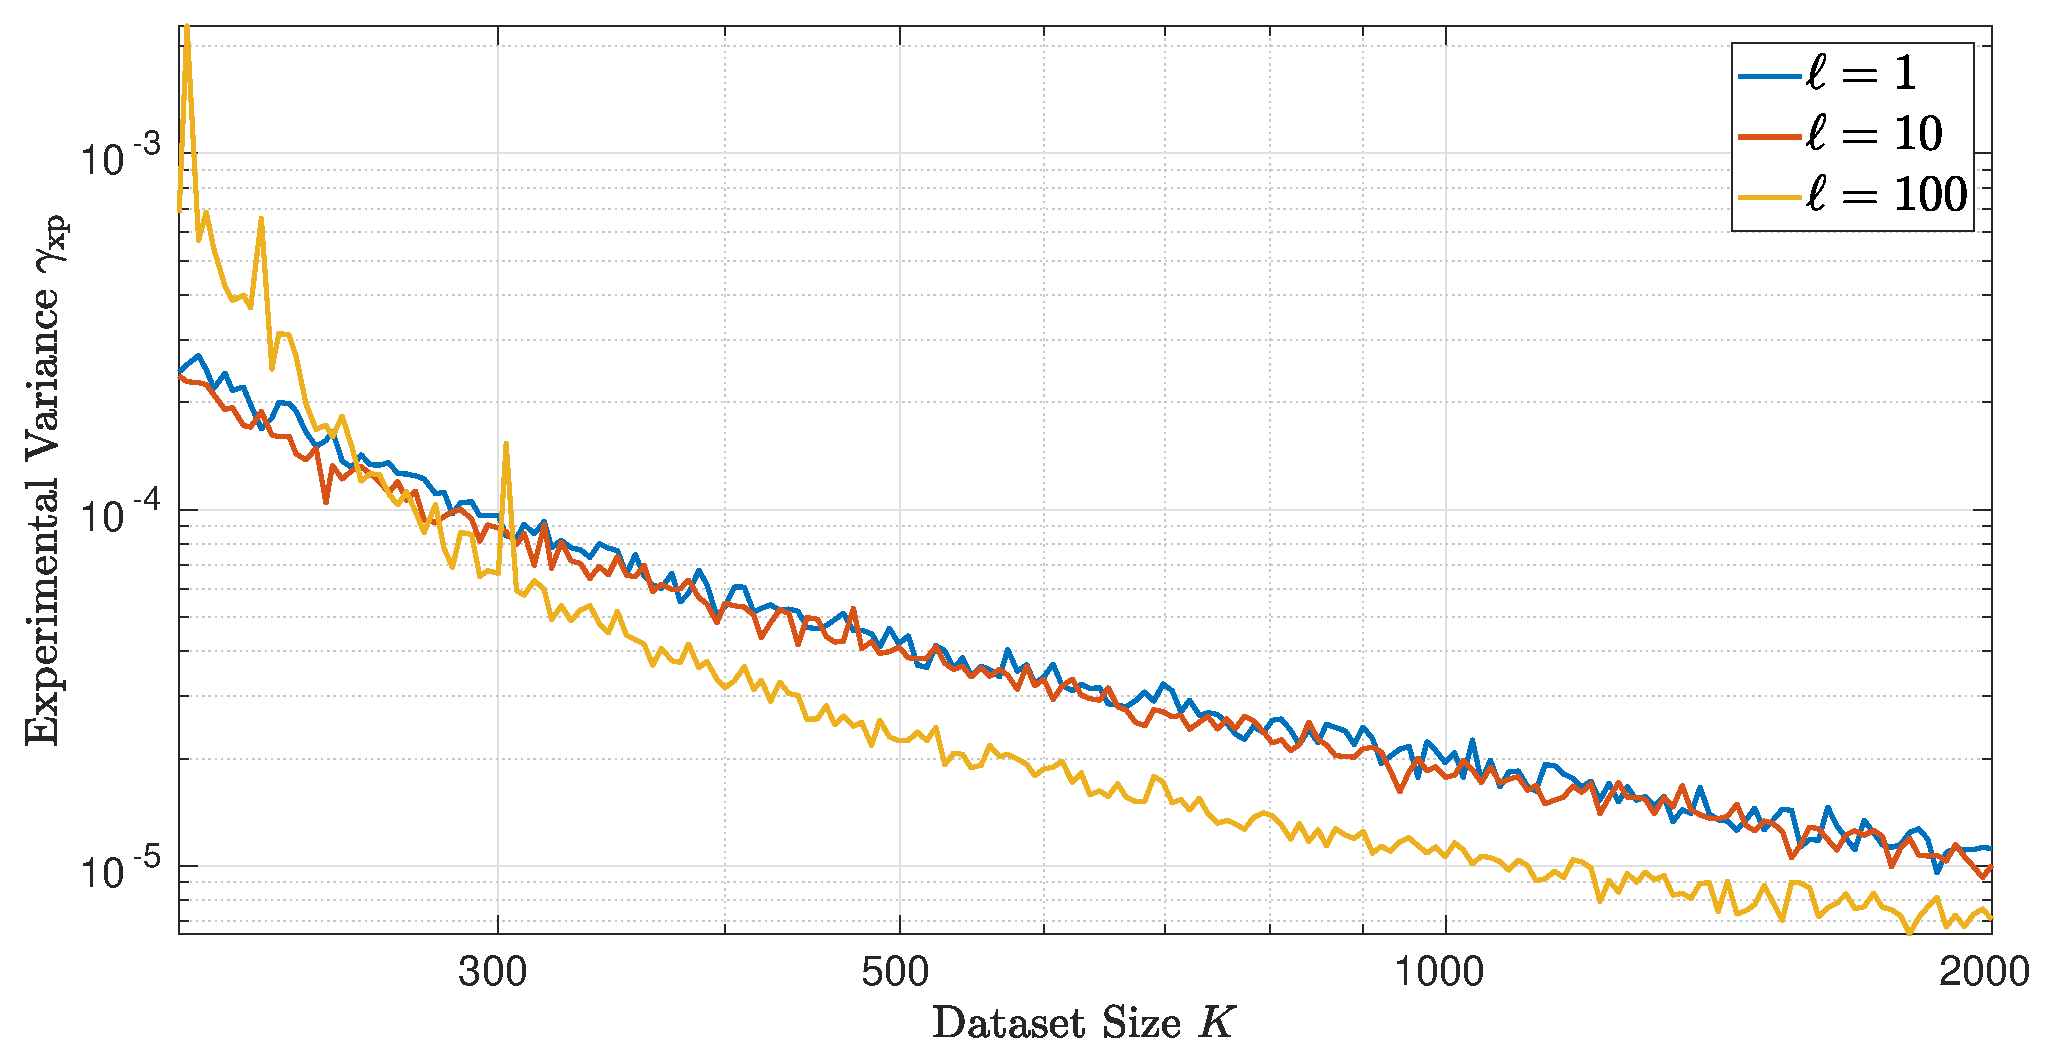
\includegraphics[width=.48\textwidth]{VarianceKSine.eps}
\caption{Evolution of the experimental forecasting variance in function of the dataset size for three different values the forecasting sample index $\ell$.}
\label{fig:res.size.sine}
\end{figure}

As anticipated by Theorem~\ref{th:error}, the variance of the estimator decreases linearly with $\frac1K$ as long as the dataset size is large enough. Indeed, in the log-log plot displayed in Fig.~\ref{fig:res.size.sine}, as soon as $K>700$, each of the three curves representing the forecasting variance as a function of $K$ tends towards an asymptote of slope $-1$. 
%
{\color{red}
In practice, the asymptotic behavior of {\sf SigExt}, illustrated here on a synthetic signal, can be generalized to the study of real-life signals, as long as the duration of the recorded signal largely exceeds that of the desired extension, which allows the user to set $K\gg L$.
}


This study overlooks the analysis of the influence of the parameter $M$, whose influence on the value of the experimental variance is numerically not significant as long as $M\ll 2K$ and $\ell<M$. The choice of this parameter is especially crucial when the deterministic component of the signal is no longer stationary. The AHM, discussed below, is an example.

\subsubsection{Adaptive Harmonic Model}
\label{ssse:res.ahm}
Consider a signal satisfying the AHM so that the instantaneous frequencies and amplitudes of its components vary over time. The deterministic component $\bz$ of the random vector $\bx$, constructed following the model~\eqref{eq:model.noise}, takes the following form, for all $n\in\{1,\ldots,N\}$:
\[
\bx[n] = \cos\left(2\pi \phi_1[n] \right) + R[n]\cos\left(2\pi \phi_2[n] \right) \ ,
\] 
where the instantaneous amplitude $R$ is given by:
\[
R[n] = 1.4 + 0.2\cos\left(4\pi\frac{n}{N}\right)\ ,
\]
and the instantaneous phases are such that:
\begin{align*}
\phi_1[n] &= \frac{p_1}{P}\left( n + \frac{0.01}{2\pi}\cos\left(2\pi\frac{n}{N}\right) \right) \\[-1mm]
\phi_2[n] & = p_2\frac{n}{P} + \frac{20}{2N\fs}n^2\ .
\end{align*}
Besides, the noise is chosen to be Gaussian, $\bw\sim\cN(\bzero,\bI)$, and we take $N=10^4$, $P=750$, $p_1=10$, $p_2=23$.

{\color{red}
\paragraph{Influence of the subsignals length $M$}
To evaluate the forecasting quality, {\sf SigExt} is applied to $1000$ realizations of the above-described signal. We forecast signal extensions of $0.1$~s, \ie~$L=700$. Table~\ref{tab:mse.sine} shows the resulting mean and standard deviation (SD) of the experimental MSE, according to four different values of the subsignals length $M$. Note that choosing a too small value for $M$ does not provide enough information to forecast the signal satisfactorily. Furthermore, a value of $M$ that is too large makes the algorithm insensitive to local nonstationarities produced by frequency variations. The user must then make a compromise on the choice of $M$ in order to optimize the performance of the algorithm. A choice of $M$ such that the subsignals contain about a dozen oscillations is generally appropriate.

\paragraph{Comparison of the extensions methods}
The same set of experiments is run on the extension methods outlined in section~\ref{sse:methods}. The results, displayed in Table~\ref{tab:mse.sine}, show that the naive extension we propose gives satisfying results. Indeed, when the subsignal length $M$ is optimally chosen, {\sf SigExt} performance is of the same order as that of ore sophisticated methods, like GPR or TBATS. Besides, even though these methods could be slightly more robust to perturbations, they are substantially limited by the computing time they require, which prevents them from being used to exploit real-time data. Thus, {\sf SigExt} is the extension method that optimizes the trade-off between forecasting quality and computing time.
Besides, the last column of Table~\ref{tab:mse.sine} gives the performance index $D$ of the boundary-free STFT associated with each extension method. This illustrates the ability of our algorithm to reduce boundary effects to a level comparable to what is possible with the GPR or TBATS extensions. The performance of {\sf BoundEffRed} on other TF representations is more thoroughly analyzed on real-life signals in the following.
}

\begin{table}
\centering
\caption{AHM Signal: Performance of the Extension Methods and the Associated Boundary-Free STFT}
\begin{tabular}{|c||c|c||c|}
  \hline
   \multirow{2}{60pt}{\centering Extension method}  & \multirow{2}{30pt}{\centering CPU time (s)} & \multirow{2}{50pt}{\centering MSE\\ (mean $\pm$ SD)} & \multirow{2}{50pt}{\centering Index $D$ of the STFT}\\
    &  & & \\
   \hhline{|=#=|=#=|}
   {\sf SigExt ($M=100$)} & $0.008$ & $1.133 \pm  0.077$ & $0.0091 \pm  0.0019$\\
   \hline
   {\sf SigExt ($M=750$)} & $0.122$ & $0.479 \pm  0.166$ & $0.0056 \pm  0.0019$\\
   \hline
   {\sf SigExt ($M\!=\!1500$)} & $0.634$ & $0.907 \pm  0.377$ & $0.0065 \pm  0.0023$\\
   \hline
   {\sf SigExt ($M\!=\!3000$)} & $2.881$ & $5.365 \pm  3.919$ & $0.0117 \pm  0.0038$\\
   \hline
   Symmetric &  $<0.001$ & $5.452 \pm  0.002$ & $1.8209 \pm  0.0025$\\
   \hline
   EDMD & $1.587$ & $0.983  \pm  0.004$ & $0.1145 \pm  0.0018$\\
   \hline
   GPR & $515.787$ & $0.479  \pm  0.166$ & $0.0119 \pm  0.0037$\\
   \hline
   TBATS  & $1776.778$ & $0.686 \pm  0.467$ & $0.3847 \pm  0.1397$\\
   \hline
\end{tabular}
\label{tab:mse.sine}
\end{table} 


\subsection{Real Physiological Signals}
\label{sse:physio.sig}


\subsubsection{Respiratory Signal}
We first consider a thoracic movement signal recorded by the piezo-electrical sensor of length 6 hours and 20 minutes. The signal is sampled at $\fs=100$~Hz. A small portion of this signal is displayed in Fig.~\ref{fig:tho}.

\begin{figure}
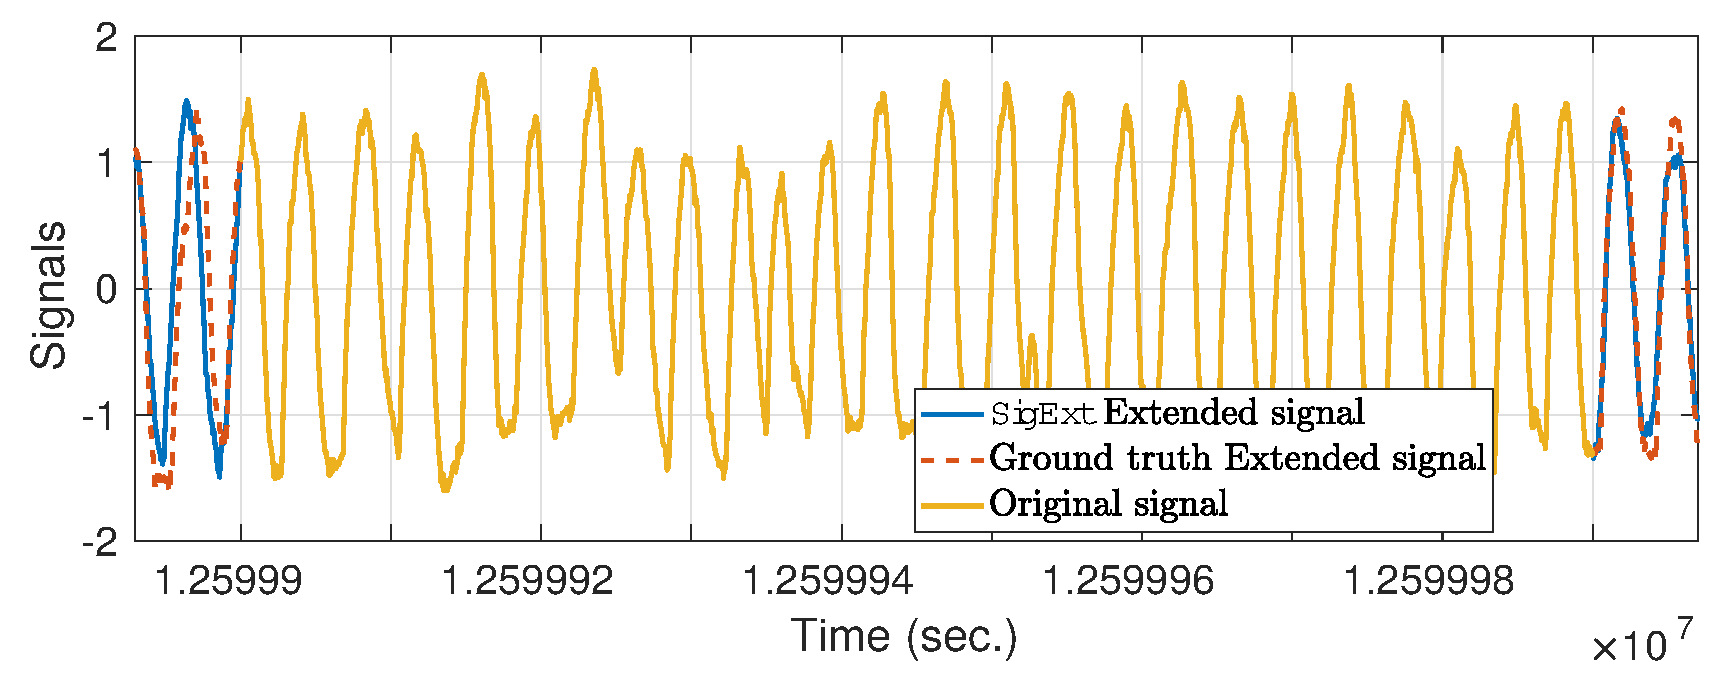
\includegraphics[width=.48\textwidth]{THOforecast.eps}
\caption{Extended respiratory signal (blue) obtained by the {\sf SigExt} forecasting (first panel), the EDMD forecasting (second panel), the GPR forecasting (third panel), and the TBATS forecasting (fourth panel), superimposed with the ground truth signal (red-dashed line).}
\label{fig:tho}
\end{figure}

From that long signal, we build a dataset of $379$ non\-overlapping signals of 60 seconds, \ie~$N=6000$. For each segment, we apply the forecasting methods introduced in section~\ref{ssse:res.ahm}, including the {\sf SigExt} method detailed in Algorithm~\ref{alg:extension}. We forecast $7$-second-long extensions on each segment of the signal, corresponding to $L =700$. Thus, in order to catch the dynamical behavior, the size of the training signal $M$ is chosen so that $M=\lfloor 1.5L\rfloor$. As a result of section~\ref{ssse:res.sine}, we take: $K=\lfloor2.5M\rfloor$. The extensions obtained on one of these subsignals are shown in Fig.~\ref{fig:tho}. The resulting MSEs of different methods are given in Table~\ref{tab:THO}. Note that the results are given in ``mean $\pm$ standard deviation'' format. The TBATS extension method is not implemented, as its excessive computing time makes it impossible to implement it on $6000$ segments within a reasonable period of time.
%
Note that the MSE of {\sf SigExt} is on average higher than the MSE of EDMD or the symmetric extension, with a huge standard deviation. This variability is caused by the presence of few segments contaminated by artifacts so that it is unpredictable via a too simple dynamical model like~\eqref{eq:dyn.model}. The left of Fig.~\ref{fig:THO.failure} illustrates one of these outliers, where {\sf SigExt} fails to catch the fast varying dynamic of the instantaneous amplitude to satisfactorily forecast the signal. The EDMD and symmetric extensions are more robust to those situations, as shown in this example, and in Table~\ref{tab:THO}. Nevertheless, {\sf SigExt} provides a sufficiently relevant extension to give TF representations sparingly affected by boundary effects. On the right of Fig.~\ref{fig:THO.failure}, we display a comparison between the right boundary of SST of the same segment of signal (top-right), and its boundary-free SST obtained after the {\sf SigExt} forecasting (bottom-right). The extension of the instantaneous frequency visible on the right side of the image illustrates the reduction of boundary effects produced despite an inaccurate signal forecasting.

We then apply {\sf BoundEffRed} for diverse TF representations: STFT, SST, RS, as well as \textit{Concentration of Frequency and Time} (ConceFT), a generalized multitaper SST-based representation introduced in~\cite{Daubechies16conceft}.  We mention that unlike other representations, the standard RS is not causal and rigorously requires knowing the STFT on the whole time-frequency plane before making any reassignment. To enable real-time implementation of RS, we use here a real-time version of RS proposed in~\cite{Lin17conceft}.

We set the extension length $L$ accordingly to the window length used by the TF analysis tool. For instance, the window length used to evaluate the STFT is of $1400$ samples. To prevent the STFT from being sensitive to the boundaries, we set $L=700$. In this way, the evaluation of the spectral content of the signal near its boundary is not limited by a lack of information in the interval delimited by the window support. From now on, all results are given for $L$ equal to the half of the width of the window used in the TF transform.
%
In Table~\ref{tab:THO}, we give the averaged performance index~\eqref{eq:index.perf} by evaluating the whole TF representations (including boundaries). Even though {\sf SigExt} performs moderately well in the sense of MSE, the boundary effects are dramatically reduced on the TF representations, and the averaged performance is in the same order of that given by EDMD or GPR. A t-test is performed to compare the performance index of {\sf SigExt} with those of other methods. Under the null hypothesis that the means are equal, with a $5\%$ significance level, the t-tests show no statistically significant difference between {\sf SigExt} and EDMD or GPR, regardless of the representation considered.


\begin{table}
\centering
\caption{Respiratory Signal: Performance of the Extension Methods and the Associated Boundary-Free TF Representations}
\begin{tabular}{|c||c||c|c|c|c|}
  \hline
   \multirow{2}{38pt}{\centering Extension method} & \multirow{2}{29pt}{\centering MSE} & \multicolumn{4}{c|}{Performance index $D$ (mean $\pm$ SD)} \\
   \cline{3-6}
      & & STFT & SST & RS & ConceFT \\
   \hhline{|=#=#=|=|=|=|}
   \multirow{2}{38pt}{\centering {\sf SigExt}} & $0.292$ & $0.370$ &  $0.408$ & $0.866$ & $0.423$ \\
   & $\pm 4.438$ & $\pm 0.623$ &  $\pm 0.436$ & $\pm 0.879$ & $\pm 0.344$ \\
   \hline
   \multirow{2}{38pt}{\centering Symmetric} & $0.044$ & $1.162$ & $1.173$ & $1.022$ & $1.144$ \\
   & $\pm 0.111$ & $\pm 0.893$ &  $\pm 0.886$ & $\pm 0.281$ & $\pm 0.579$ \\
   \hline
   \multirow{2}{38pt}{\centering EDMD} & $0.026$ & $0.359$ &  $0.422$ & $0.828$ & $0.449$ \\
   & $\pm 0.112$ & $\pm 0.266$ &  $\pm 0.282$ & $\pm 0.248$ & $\pm 0.296$ \\
   \hline
   \multirow{2}{38pt}{\centering GPR} & $0.331$ & $0.391$ &  $0.411$ & $0.897$ & $0.430$ \\ 
   & $\pm 4.858$ & $\pm 0.853$ &  $\pm 0.406$ & $\pm 1.140$ & $\pm 0.364$ \\
   \hline
\end{tabular}
\label{tab:THO}
\end{table}

\begin{figure}
\centering
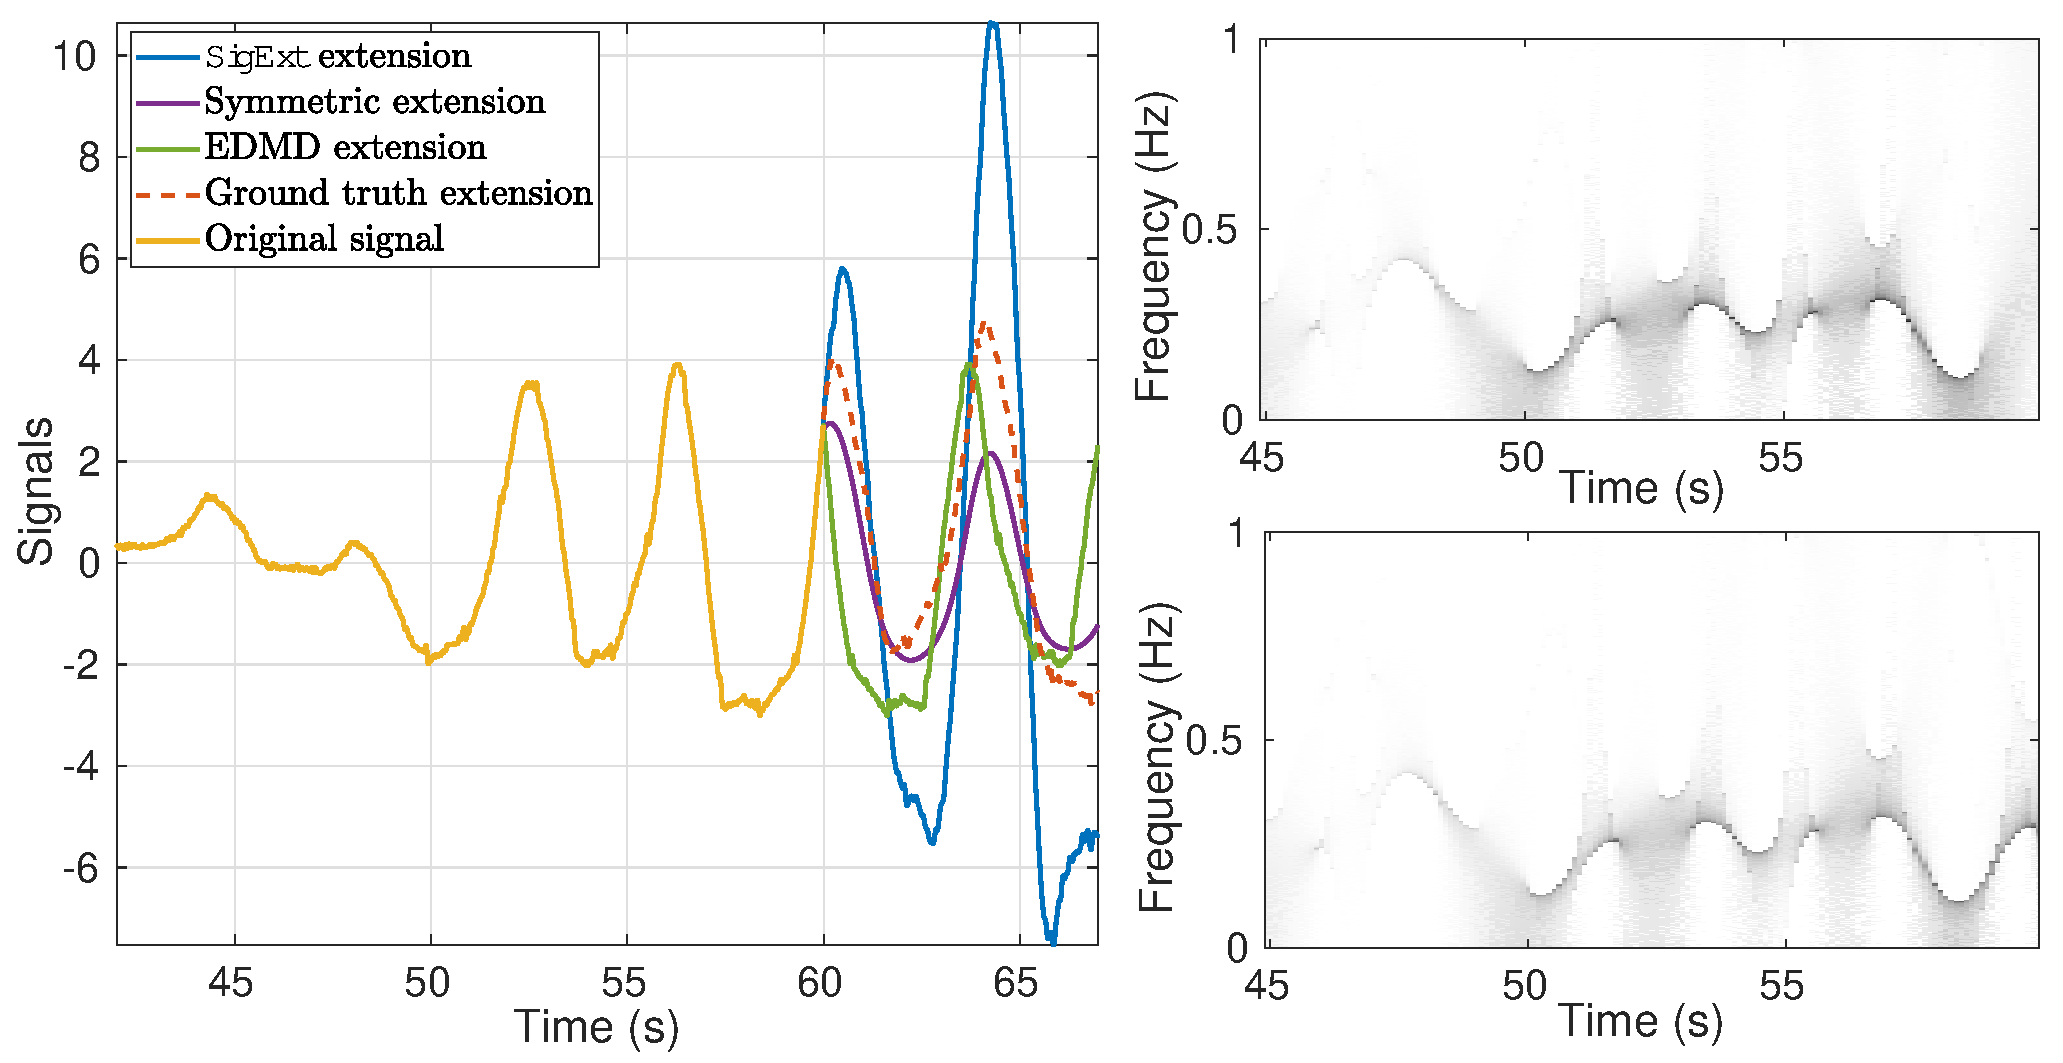
\includegraphics[width=.48\textwidth]{THOfailure.eps}
\caption{Extensions of a segment of the respiratory signal (left) where {\sf SigExt} is outperformed by the EDMD and Symmetric extensions. Corresponding SST (top-right) and boundary-free SST obtained with {\sf SigExt} (bottom-right).}
\label{fig:THO.failure}
\end{figure} 

{\color{red}
Then, we consider a second respiratory signal that contains not only the respiratory cycle, but also the cardiogenic artifact which reflects the hemodynamic component. Fig.~\ref{fig:resp.2} displays the boundary-free SST of a 180-second-long extract of this signal, sample at $125$~Hz, obtained via {\sf BoundEffRed}. This TF analysis brings out both components---the respiratory component, the most energetic, is located around the fundamental frequency $0.25$~Hz and its multiples, while the cardiac component, less visible, is located around $1.7$~Hz. The performance index of this representation takes the value $D=0.314$. Note that, here, boundary effects are only reduced on the right-side boundary of the TF domain. This means that {\sf BoundEffRed} has reduced the right-side boundary effects by about $69\%$ with respect to the ordinary SST. This shows the ability of our algorithm to work on signals containing several nonstationary components.

\begin{figure}
\centering
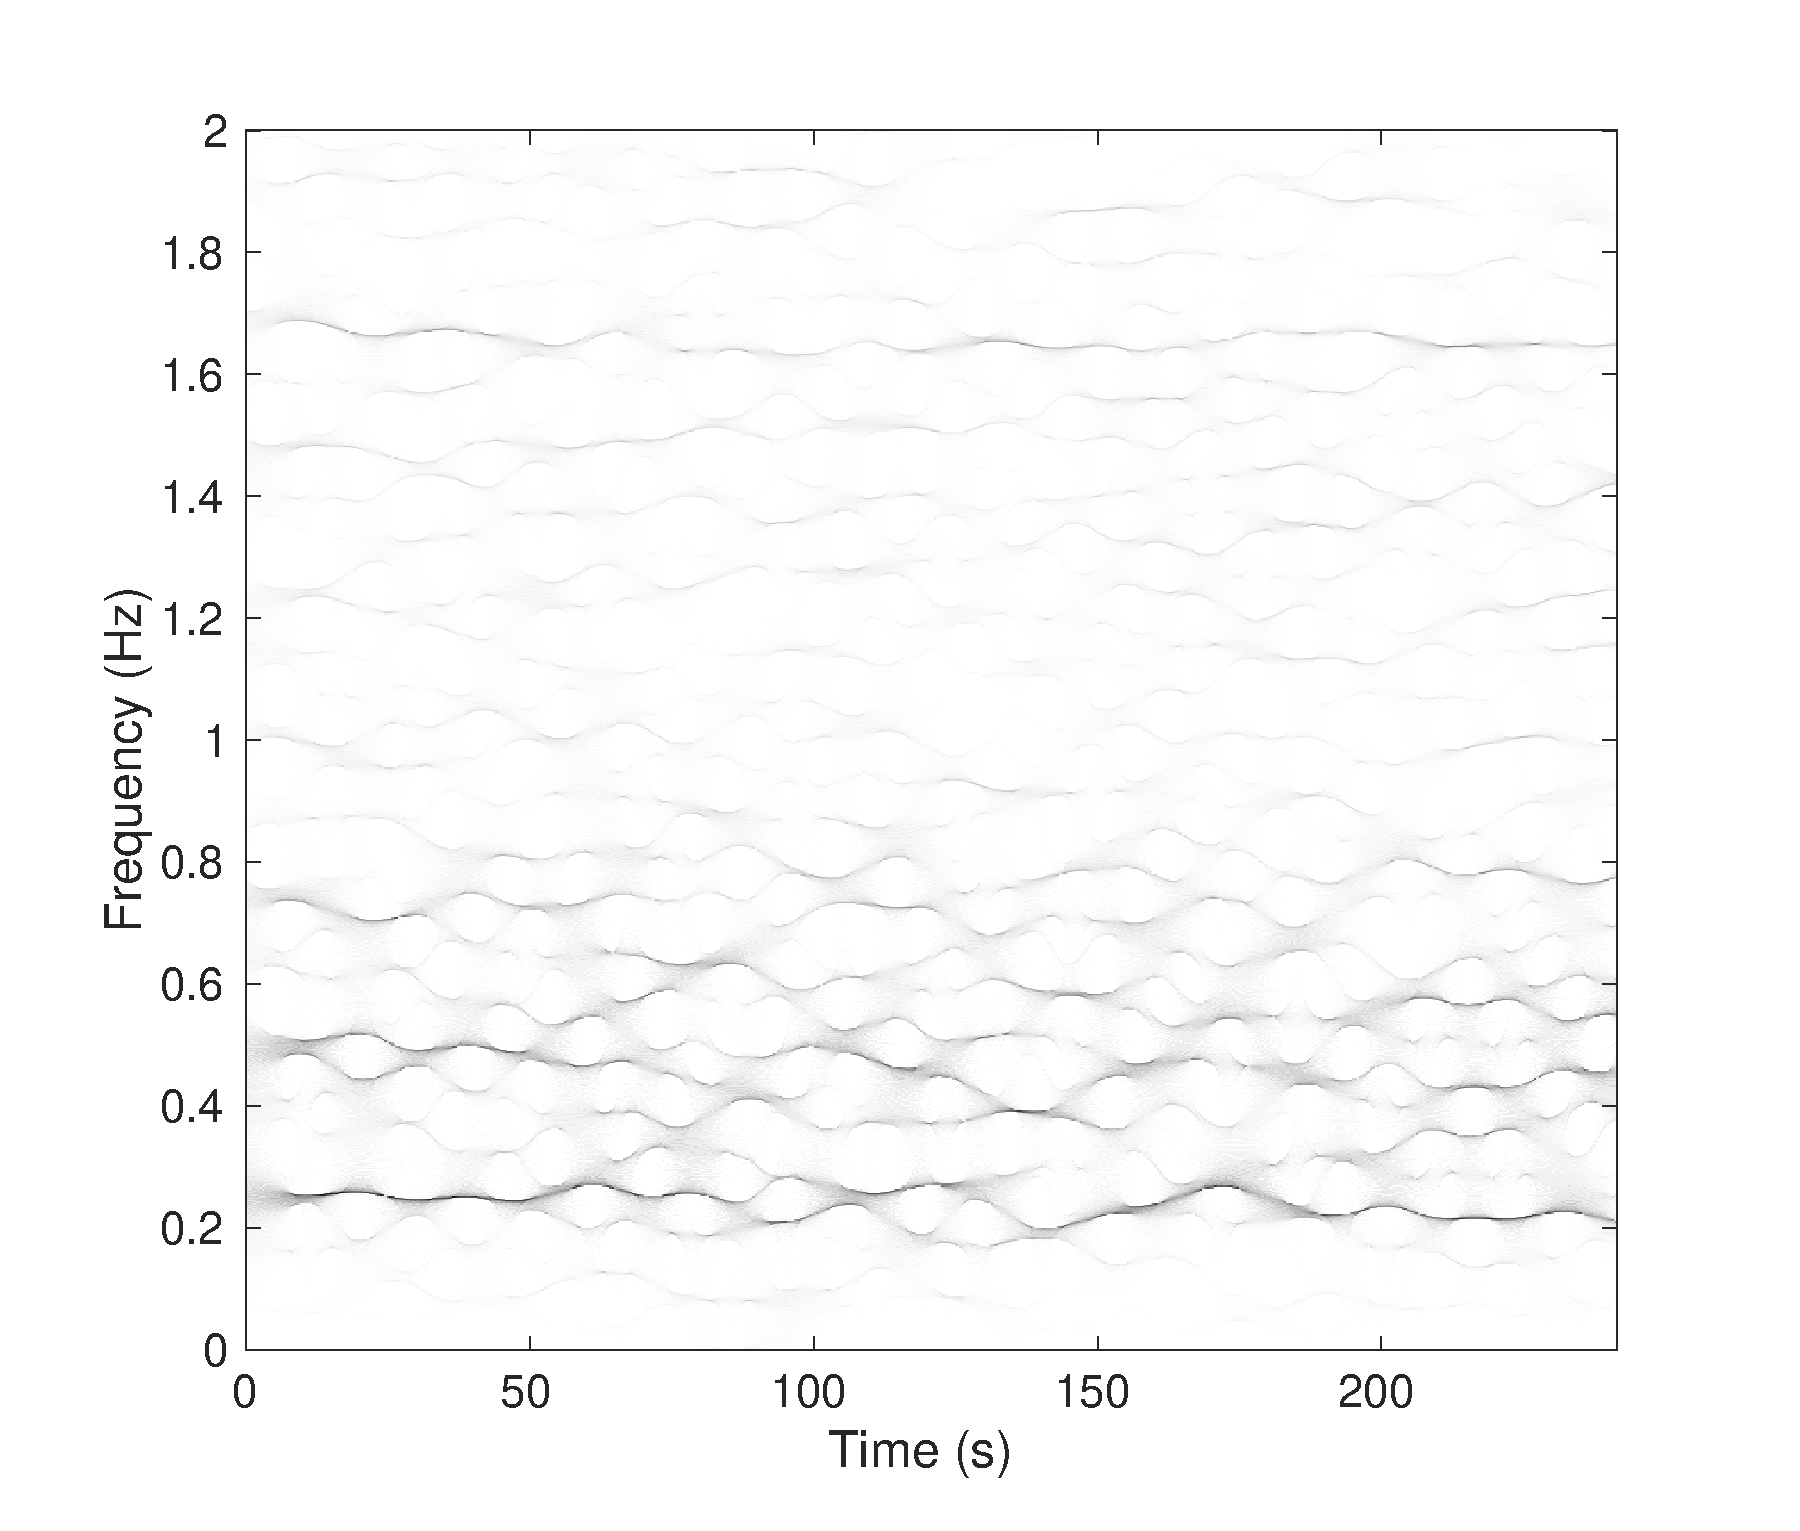
\includegraphics[width=.48\textwidth]{Resp2comp.eps}
\caption{Boundary-free SST of a two-component respiratory signal.}
\label{fig:resp.2}
\end{figure} 
}

\subsubsection{Photoplethysmogram}
\label{ssse:ppg}
We perform a study similar to the previous one on a $640$-second-long photoplethysmogram (PPG) signal extracted from the Physionet dataset~\cite{Pimentel17toward, Goldberger00physiobank}, sampled at $\fs=125$~Hz. A portion of this signal is displayed in Fig.~\ref{fig:ppg}. The estimated 5 seconds extensions of this segment obtained by {\sf SigExt}, EDMD, and GPR forecastings  are superimposed to the ground-truth extension in Fig.~\ref{fig:ppg}.

\begin{figure}
%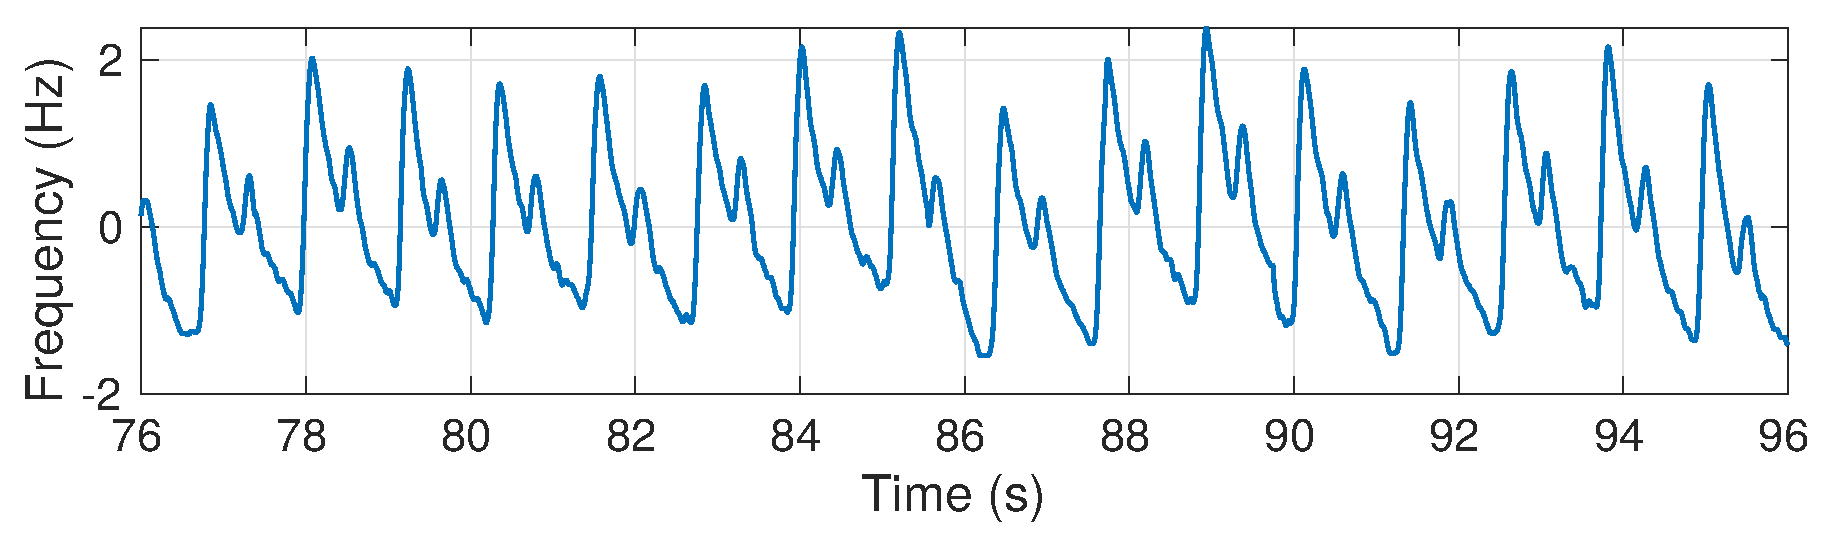
\includegraphics[width=.48\textwidth]{PPGsig.eps}
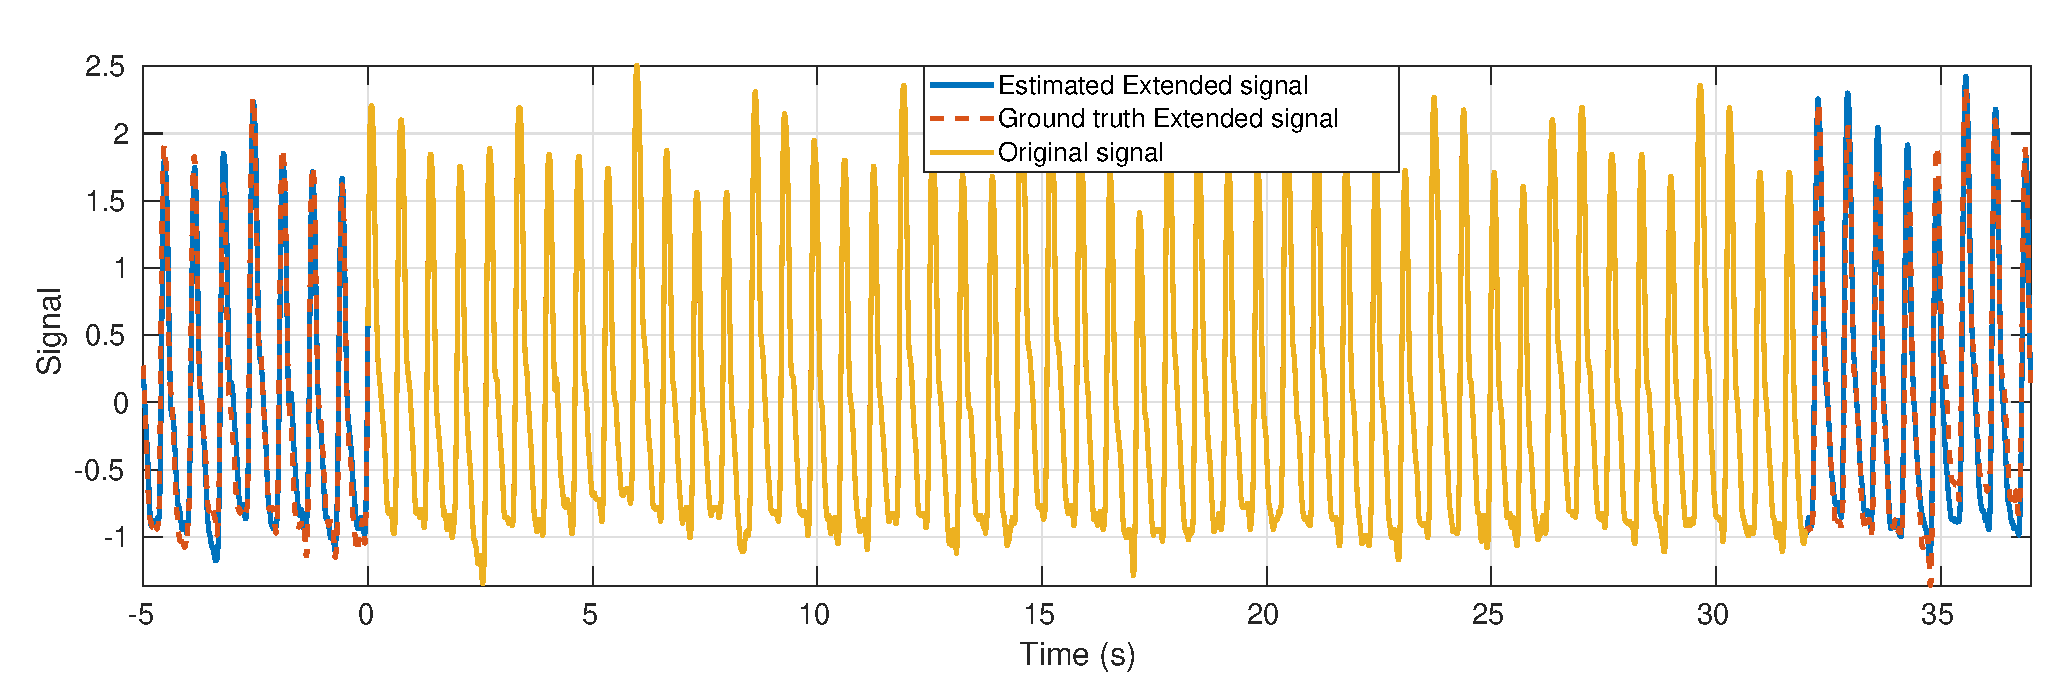
\includegraphics[width=.48\textwidth]{PPGforecast.eps}
\caption{Extended PPG signal (blue) obtained by the {\sf SigExt} forecasting (top), the EDMD forecasting (middle), and the GPR forecasting (bottom), superimposed with the ground truth signal (red dash).}
\label{fig:ppg}
\end{figure}

We divide the signal into 32-second-long segments and apply {\sf BoundEffRed} to each of them. Table~\ref{tab:otd.ppg} shows the performance index $D$ of the boundary-free TF representations, averaged over the signals. For all the TF representations considered, the results show that {\sf SigExt} reduces boundary effects about as efficiently as the extensions given by EDMD or GPR. As for the respiratory signal, t-tests show no statistically significant difference between {\sf SigExt} and EDMD or GPR, regardless of the representation considered. For visual inspection, the TF representation of SST resulting from the {\sf BoundEffRed} strategy is shown in the bottom-right panel of Fig.~\ref{fig:ex.intro}, where SST is applied to the portion of PPG displayed in Fig.~\ref{fig:ppg}. It produces a significant improvement in the quality of the SST near boundaries. Indeed, the blurring visible when zooming on the right boundary of the SST has almost vanished. Real-time tracking of the instantaneous frequencies contained in the measured signal is therefore greatly facilitated.

\begin{table}
\centering
\caption{PPG Signal: Performance of the Boundary-Free TF Representations According to the Extension Method}
\begin{tabular}{|c||c||c|c|c|c|}
  \hline
   \multirow{2}{38pt}{\centering Extension method} & \multirow{2}{29pt}{\centering MSE} &\multicolumn{4}{c|}{Performance index $D$ (mean $\pm$ SD)} \\
   \cline{3-6}
      & & STFT & SST & ConceFT & RS\\
   \hhline{|=#=#=|=|=|=|}
   \multirow{2}{38pt}{\centering {\sf SigExt}} & $0.018$ & $0.280$ & $0.309$ & $0.367$ & $0.534$ \\
    & $\pm 0.014$ & $\pm 0.107$ & $\pm 0.112$ & $\pm 0.183$ & $\pm 0.160$ \\
   \hline
   \multirow{2}{38pt}{\centering Symmetric} & $0.037$ & $1.168$ & $1.209$ & $1.310$ & $0.983$ \\
   & $\pm 0.007$ & $\pm 0.390$ & $\pm 0.340$ & $\pm 0.140$ & $\pm 0.304$ \\
   \hline
   \multirow{2}{38pt}{\centering EDMD} & $0.012$ & $0.289$ & $0.319$ & $0.375$ & $0.503$ \\
   & $\pm 0.005$ & $\pm 0.126$ & $\pm 0.134$ & $\pm 0.163$ & $\pm 0.163$ \\
   \hline
   \multirow{2}{38pt}{\centering GPR} & $0.018$ & $0.276$ & $0.303$ & $0.361$ & $0.544$ \\
   & $\pm 0.013$ & $\pm 0.106$ & $\pm 0.110$ & $\pm 0.165$ & $\pm 0.157$ \\
   \hline
\end{tabular}
\label{tab:otd.ppg}
\end{table}

To further evaluate the influence of the noise level on the performance of {\sf BoundEffRed}, we artificially add Gaussian noise to the measured PPG signal. It is thus an additional noise to the measurement noise actually contained in the signal. Fig.~\ref{fig:otd.noise} shows the average performance index of {\sf BoundEffRed} for different values of the Signal-to-Noise Ratio (SNR). Whatever the representation considered, {\sf BoundEffRed} is relatively robust to noise, as long as the SNR remains above $10$~dB. Below this level, the reduction of boundary effects gradually deteriorates.

\begin{figure}
\centering
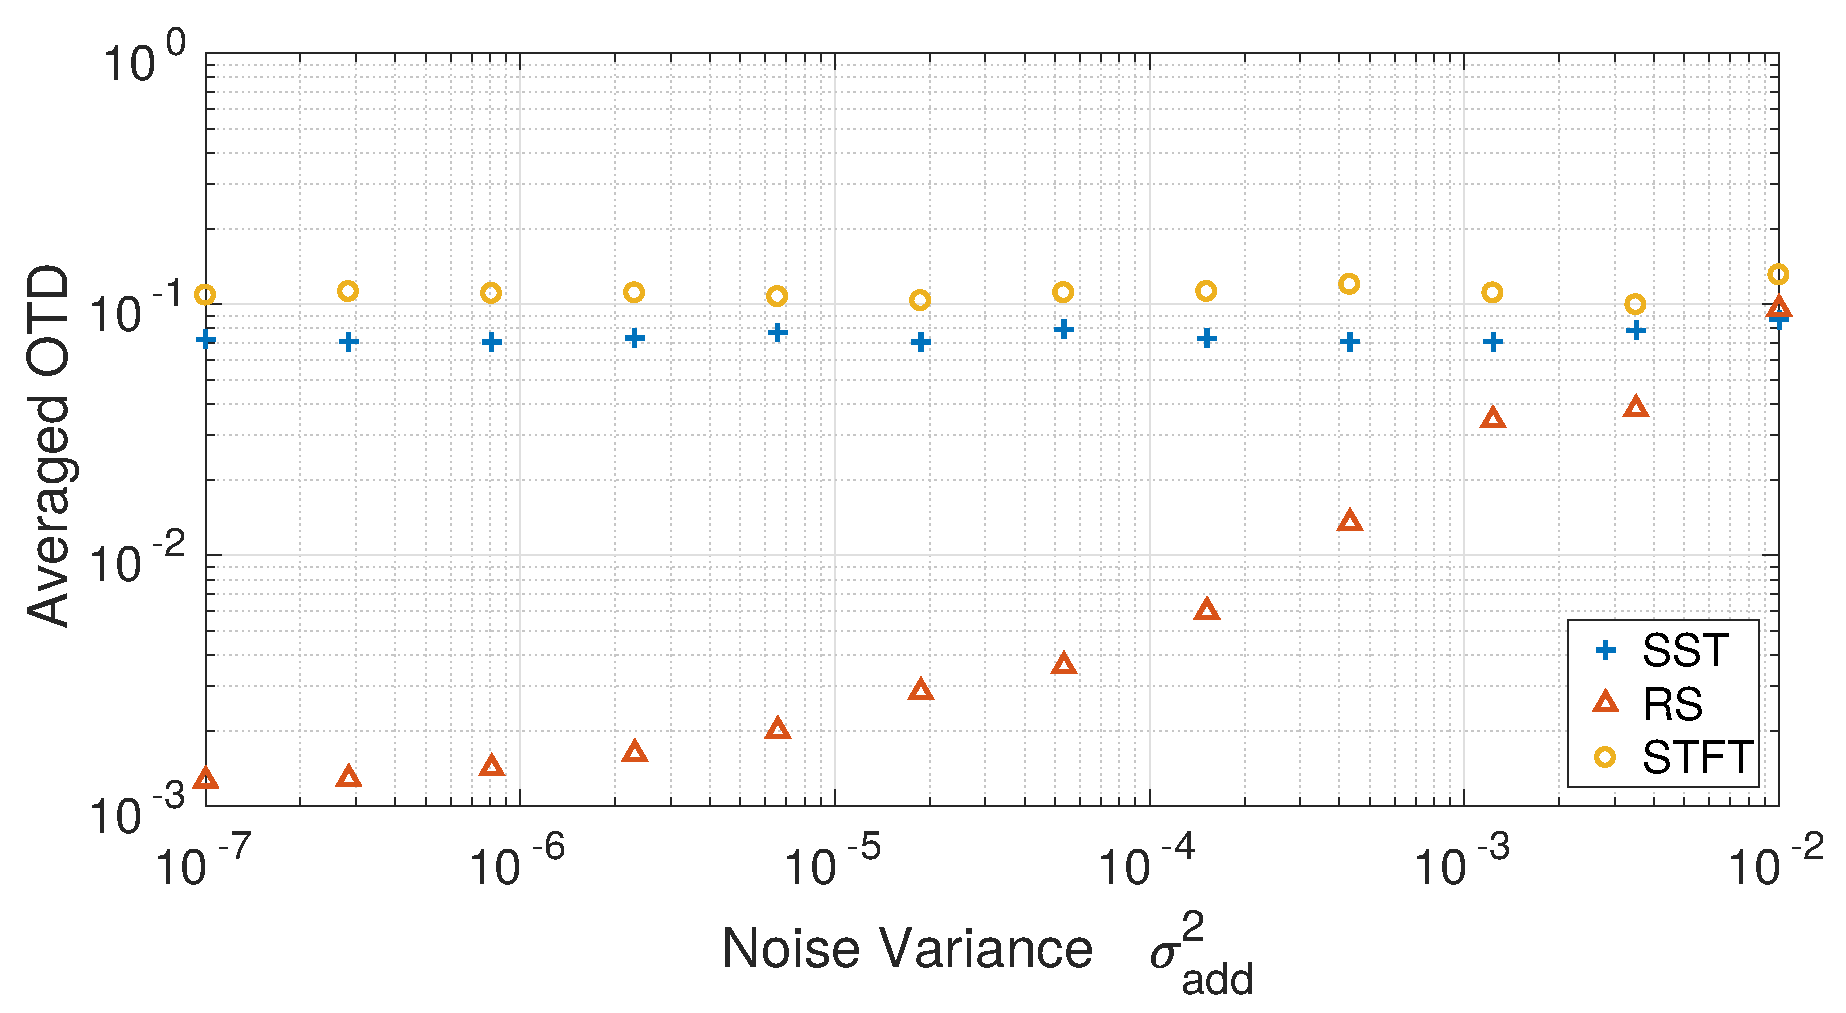
\includegraphics[width=.48\textwidth]{OTDBoundEffRed.eps}
\caption{Performance index of {\sf BoundEffRed} applied on a PPG, in function of the SNR.}
\label{fig:otd.noise}
\end{figure}


\subsection{Real-Time Implementation}
We simulate the real-time implementation of the SST from {\sf BoundEffRed} applied to the PPG described in section~\ref{ssse:ppg}, subsampled by a factor of $2$. The test is performed on a 2-Core Intel Core i5 CPU running at $1.7$~GHz and $7.7$~GB of RAM. 

For this signal, sampled at $\fs=65.5$~Hz, the suitable window is $8$ seconds long. Therefore, the extension must be over $4$ seconds, \ie~$L=250$. The forecasting step in each iteration of {\sf BoundEffRed} then takes no more than $t_{\mathrm{forecast}}=46$~ms. Denote by $H\geq 1$ the hop size in samples, that is the number of samples between successive columns of the SST. Besides, since the support of the analysis window covers $2L$ samples, the update of the SST requires the calculation of $\lceil 2L/H \rceil$ new columns of the SST. In this example, the frequency dimension of the SST being $512$, the computational time of one column is $t_{\mathrm{SST}}=2.08$~ms, on average. A general rule to determine the acceptable values of $H$ for real-time implementation is verifying that the computational time to update the boundary-free TF representation is smaller than the lag between $H$ samples; that is,
\[
t_{\mathrm{forecast}} + \left\lceil \frac{L}H \right\rceil t_{\mathrm{SST}} < \frac{H}\fs\ . 
\]
In our example, taking $H\geq 8$~samples is sufficient to ensure the feasibility of real-time implementation. This value is reasonable because it allows a maximum overlap of $98.4\%$ of the window length. SST variations are therefore perceived gradually. Combined with the low latency of the algorithm, this allows for smooth monitoring of the real-time SST. A video clip illustrating this is available on GitHub, at \url{https://github.com/AdMeynard/BoundaryEffectsReduction/tree/master/Animations}. 